\refstepcounter{section}
\section*{Lecture 16: Kink Solutions}
\addcontentsline{toc}{section}{Lecture 16: Kink Solutions}
In the previous lecture, we introduced a spatial variation of the order parameter, $m(\vb{x})$. Consider the 1D Ising chain as an example. Suppose in the extreme left end of the chain, we have a $\uparrow$ spin while in the extreme right, we have a $\downarrow$ spin.\\[0.2cm] If we keep this constraint, then it is evident that somewhere in the middle, there should be a spin flip (that is, we cannot \textit{continuously deform} the left side to bring it to the right side). This inability to continuously deforma aptly indicates that this is a \textit{topological artifact}. \\[0.2cm]
This spin flip is nothing but a \textit{domain wall} if we think about it. The domain wall is also exotically called a \textit{kink} or \textit{soliton} depending on the context and the type of system used. Note that if there are two kinks, then there are two spin flips and hence these cancel each other (that is, the boundaries have the same spins). Thus, this configuration can be continuously deformed to the ground state. 
\begin{figure}[H]
    \begin{center}
        

\tikzset{every picture/.style={line width=0.75pt}} %set default line width to 0.75pt        

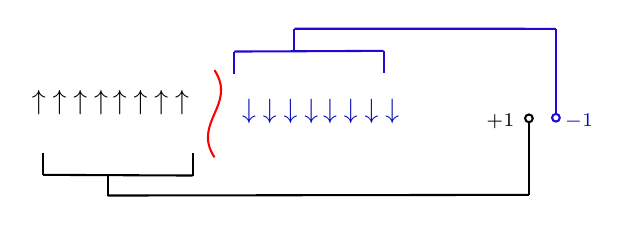
\begin{tikzpicture}[x=0.75pt,y=0.75pt,yscale=-1,xscale=1]
%uncomment if require: \path (0,300); %set diagram left start at 0, and has height of 300

%Curve Lines [id:da11923680593337727] 
\draw [color={rgb, 255:red, 255; green, 0; blue, 0 }  ,draw opacity=1 ]   (231.51,69.65) .. controls (242.5,86.45) and (220.52,94.85) .. (231.51,111.65) ;
%Straight Lines [id:da38427999729120976] 
\draw    (149,120.08) -- (221,120.42) ;
%Straight Lines [id:da19236732945789958] 
\draw    (221,109.68) -- (221,120.42) ;
%Straight Lines [id:da7562185270979398] 
\draw    (149,109.35) -- (149,120.08) ;
%Straight Lines [id:da22209538028495435] 
\draw [color={rgb, 255:red, 33; green, 10; blue, 206 }  ,draw opacity=1 ]   (241,60.68) -- (313,60.35) ;
%Straight Lines [id:da8931202046154221] 
\draw [color={rgb, 255:red, 33; green, 10; blue, 206 }  ,draw opacity=1 ]   (313,71.08) -- (313,60.35) ;
%Straight Lines [id:da5226821210184597] 
\draw [color={rgb, 255:red, 33; green, 10; blue, 206 }  ,draw opacity=1 ]   (241,71.42) -- (241,60.68) ;
%Straight Lines [id:da29426316212604653] 
\draw    (180,130.05) -- (383,129.72) ;
%Straight Lines [id:da5498785267596156] 
\draw    (180,120.32) -- (180,130.05) ;
%Straight Lines [id:da03512399816424894] 
\draw [color={rgb, 255:red, 33; green, 10; blue, 206 }  ,draw opacity=1 ]   (270,49.68) -- (396,49.72) ;
%Straight Lines [id:da2575162851855418] 
\draw [color={rgb, 255:red, 33; green, 10; blue, 206 }  ,draw opacity=1 ]   (270,60.42) -- (270,49.68) ;
%Straight Lines [id:da6286004187607146] 
\draw [color={rgb, 255:red, 33; green, 10; blue, 206 }  ,draw opacity=1 ]   (396,90.72) -- (396,49.72) ;
%Straight Lines [id:da19564964938004337] 
\draw    (383,94.72) -- (383,129.72) ;
%Shape: Circle [id:dp11637717033709771] 
\draw   (381.14,92.86) .. controls (381.14,91.83) and (381.97,91) .. (383,91) .. controls (384.03,91) and (384.86,91.83) .. (384.86,92.86) .. controls (384.86,93.88) and (384.03,94.72) .. (383,94.72) .. controls (381.97,94.72) and (381.14,93.88) .. (381.14,92.86) -- cycle ;
%Shape: Circle [id:dp5272974229423903] 
\draw  [color={rgb, 255:red, 33; green, 11; blue, 207 }  ,draw opacity=1 ] (394.14,92.57) .. controls (394.14,91.55) and (394.97,90.72) .. (396,90.72) .. controls (397.03,90.72) and (397.86,91.55) .. (397.86,92.57) .. controls (397.86,93.6) and (397.03,94.43) .. (396,94.43) .. controls (394.97,94.43) and (394.14,93.6) .. (394.14,92.57) -- cycle ;

% Text Node
\draw (142,77.62) node [anchor=north west][inner sep=0.75pt]    {$\uparrow $};
% Text Node
\draw (162,77.62) node [anchor=north west][inner sep=0.75pt]    {$\uparrow $};
% Text Node
\draw (152,77.62) node [anchor=north west][inner sep=0.75pt]    {$\uparrow $};
% Text Node
\draw (172,77.62) node [anchor=north west][inner sep=0.75pt]    {$\uparrow $};
% Text Node
\draw (181,77.62) node [anchor=north west][inner sep=0.75pt]    {$\uparrow $};
% Text Node
\draw (201,77.62) node [anchor=north west][inner sep=0.75pt]    {$\uparrow $};
% Text Node
\draw (191,77.62) node [anchor=north west][inner sep=0.75pt]    {$\uparrow $};
% Text Node
\draw (211,77.62) node [anchor=north west][inner sep=0.75pt]    {$\uparrow $};
% Text Node
\draw (253,96.82) node [anchor=north east][inner sep=0.75pt]  [color={rgb, 255:red, 7; green, 14; blue, 182 }  ,opacity=1 ,rotate=-180,xscale=-1]  {$\uparrow $};
% Text Node
\draw (273,96.82) node [anchor=north east][inner sep=0.75pt]  [color={rgb, 255:red, 7; green, 14; blue, 182 }  ,opacity=1 ,rotate=-180,xscale=-1]  {$\uparrow $};
% Text Node
\draw (263,96.82) node [anchor=north east][inner sep=0.75pt]  [color={rgb, 255:red, 7; green, 14; blue, 182 }  ,opacity=1 ,rotate=-180,xscale=-1]  {$\uparrow $};
% Text Node
\draw (283,96.82) node [anchor=north east][inner sep=0.75pt]  [color={rgb, 255:red, 7; green, 14; blue, 182 }  ,opacity=1 ,rotate=-180,xscale=-1]  {$\uparrow $};
% Text Node
\draw (292,96.82) node [anchor=north east][inner sep=0.75pt]  [color={rgb, 255:red, 7; green, 14; blue, 182 }  ,opacity=1 ,rotate=-180,xscale=-1]  {$\uparrow $};
% Text Node
\draw (312,96.82) node [anchor=north east][inner sep=0.75pt]  [color={rgb, 255:red, 7; green, 14; blue, 182 }  ,opacity=1 ,rotate=-180,xscale=-1]  {$\uparrow $};
% Text Node
\draw (302,96.82) node [anchor=north east][inner sep=0.75pt]  [color={rgb, 255:red, 7; green, 14; blue, 182 }  ,opacity=1 ,rotate=-180,xscale=-1]  {$\uparrow $};
% Text Node
\draw (322,96.82) node [anchor=north east][inner sep=0.75pt]  [color={rgb, 255:red, 7; green, 14; blue, 182 }  ,opacity=1 ,rotate=-180,xscale=-1]  {$\uparrow $};
% Text Node
\draw (361,89.4) node [anchor=north west][inner sep=0.75pt]  [font=\scriptsize]  {$+1$};
% Text Node
\draw (398.86,89.26) node [anchor=north west][inner sep=0.75pt]  [font=\scriptsize,color={rgb, 255:red, 5; green, 8; blue, 201 }  ,opacity=1 ]  {$-1$};


\end{tikzpicture}

    \end{center}
\end{figure}
\noindent
The spins left and right of the kink can be mapped from the real space (of the lattice) to the order-parameter space, where there are two points $+1$ and $-1$, as shown above. Thus a state $(+,+)$ or $(-,-)$ will have all up spins and down spins respectively and hence are the ground states. The state $(+,-)$ ( state $(-,+)$) will have up spins on the left (right) and down spins on the right (left) of the kink. These are the four topologically distinct sectors for the 1D Ising model. The state $(-,+)$ is called the kink state where we have up spins on the right of the chain while $(+,-)$ is called the anti-kink state.\\[0.2cm]
We want to see the variation of the order parameter across the domain wall. For this, consider the following Landau functional, 
\begin{equation*}
    \SL[m(\vb{x})] = \int \dd^d x \ \qty[\frac{1}{2}a_2(T-T_c)(m(\vb{x}))^2 + \frac{1}{4}a_4 (m(\vb{x}))^4 - h(\vb{x})m(\vb{x}) +\frac{\gamma}{2}\qty(\grad m(\vb{x}))^2]
\end{equation*}
Now, suppose spatial variations persist only in one direction, while all the other $(d-1)$ dimensions are spatially uniform. Hence $m(\vb{x}) \equiv m(x)$ and let $A$ be the integral over the rest of the spatially uniform $(d-1)$ dimensions (hence $A \sim l^{d-1}$).
\begin{equation}
    \frac{\SL}{A} = \int \dd x \ \qty[\frac{1}{2}a_2(T-T_c)(m(x))^2 + \frac{1}{4}a_4 (m(x))^4 - h(x)m(x) +\frac{\gamma}{2}\qty(\pdv{m(x)}{x})^2]
\end{equation}
Considering $h(x)=0$, we get the equation of motion:
\begin{equation}\label{eos}
    \gamma \dv[2]{m}{x} = a_2(T-T_c)m + a_4m^3
\end{equation}
Multiplying both sides by $\dv{m}{x}$ we get,
\begin{align*}
    {\gamma}\qty(\dv{m}{x}) \dv[2]{m}{x} = \qty[a_2(T-T_c)m + a_4m^3]\qty(\dv{m}{x})\implies &\frac{\gamma}{2}\dv{x}\qty(\dv{m}{x})^2 =\pdv{x} \qty[\frac{1}{2}a_2(T-T_c)m^2 + \frac{1}{4}a_4 m^4]\\
   \implies & \dv{x}\qty[\frac{\gamma}{2}\qty(\dv{m}{x})^2 - \frac{1}{2}a_2(T-T_c)m^2 - \frac{1}{4}a_4 m^4] =0\\
   \implies & -\frac{\gamma}{2}\qty(\dv{m}{x})^2 + \frac{1}{2}a_2(T-T_c)m^2 + \frac{1}{4}a_4 m^4 = C
\end{align*}
where $C$ is a constant determined by the boundary conditions. So let's set $m(x\to +\infty) = m_\infty = \sqrt{-\frac{a_2}{a_4}(T-T_c)}>0$ and $\dv{m}{x}\Big|_{\infty} = 0$. Using this, we obtain the value of $C$ 
\begin{align*}
    C = \frac{1}{2}a_2(T-T_c) \times \qty(-\frac{a_2(T-T_c)}{a_4}) + \frac{1}{4}a_4\times \frac{(a_2(T-T_c))^2}{a_4^2} =- \frac{[a_2(T-T_c)]^2}{4a_4}
\end{align*}
Substituting this value above, we get the equation as, 
\begin{align}
   \begin{split}
     0 &=-\frac{\gamma}{2}\qty(\dv{m}{x})^2 + \frac{1}{2}a_2(T-T_c)m^2 + \frac{1}{4}a_4 m^4 + \frac{[a_2(T-T_c)]^2}{4a_4}\\
    &=-\frac{\gamma}{2}\qty(\dv{m}{x})^2 + \frac{a_4}{4}\qty[\frac{2a_2}{a_4}(T-T_c)m^2 + m^4 + m_\infty^4]\\
    &=-\frac{\gamma}{2}\qty(\dv{m}{x})^2 + \frac{a_4}{4}\qty[-2m^2m_\infty^2+m^4 + m_\infty^4]\\
    &=-\frac{\gamma}{2}\qty(\dv{m}{x})^2 + \frac{a_4}{4}\qty(m^2-m_\infty^2)^2
   \end{split}
\end{align}
from which get two solutions, 
$$\sqrt{\frac{2\gamma}{a_4}}\dv{m}{x} = \pm (m^2-m_\infty^2)$$
We take the $-$ve solution and then we integrate to get,
$$\sqrt{\frac{2\gamma}{a_4}} \int\limits_{m(x\tund{0})}^m \frac{\dd m}{m_\infty^2-m^2} = \int\limits_{x\tund{0}}^x \dd x = (x-x\tund{0})$$
where $x\tund{0}$ is the centre of the domain wall and we assume $m(x\tund{0}) = 0$. On solving the integral, we obtain the solution, 
\begin{align*}
    \sqrt{\frac{2\gamma}{a_4}} \frac{1}{m_\infty}\tanh^{-1}\qty(\frac{m}{m_\infty})= (x-x\tund{0})\implies m(x) &= m_\infty \tanh\qty[\frac{m_\infty(x-x\tund{0})}{\sqrt{2}\qty(\gamma/a_4)^{1/2}}]\\&= m_\infty \tanh\qty[\frac{(x-x\tund{0})}{\sqrt{2}\mathcolor{red}{\qty(\gamma/a_4)^{1/2}\qty(a_2(T_c-T)/a_4)^{-1/2}}}]
\end{align*}
Now, the red quantity has the dimension of length and we denote is by $\xi$. Physically, $\xi$ denotes the length scale over which significant change occurs across the domain wall. This is appropriately called the \textit{correlation length} since this is the scale across which correlations between the spins persist. The correlation length is temperature dependent as seen above. It scales as, $\xi \sim (T_c-T)^{-1/2}$, hence shows a power-law divergence at $T=T_c$.
\begin{figure}[H]
    \centering
    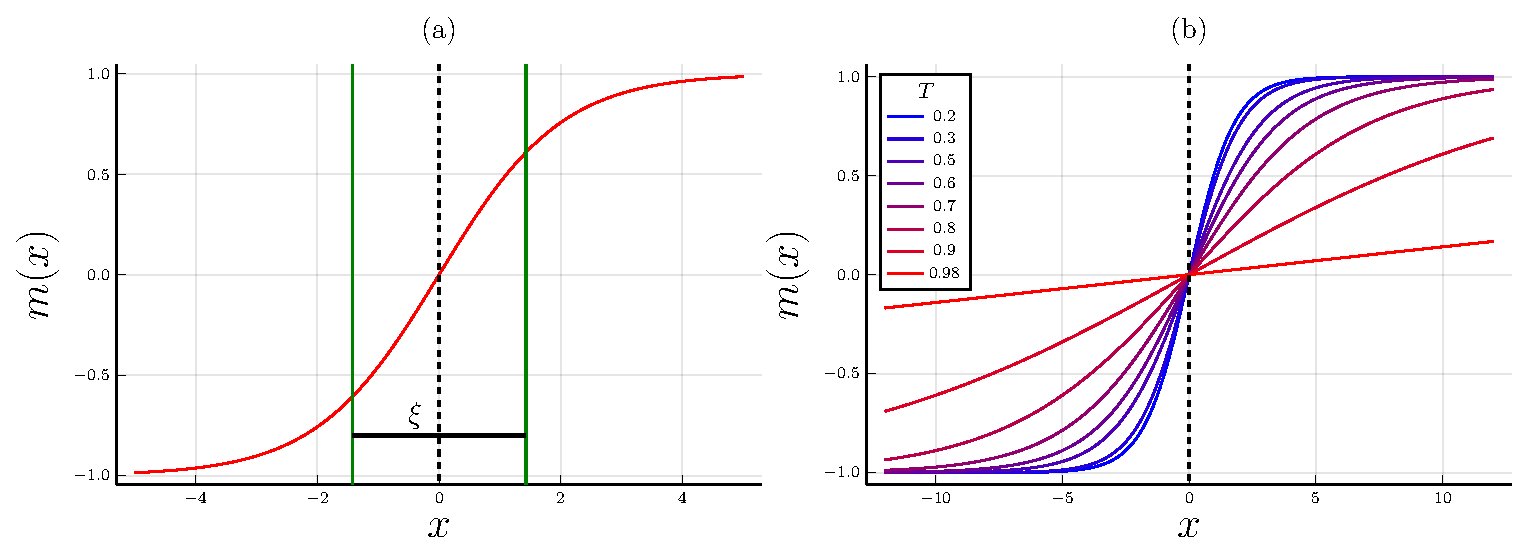
\includegraphics[width=\textwidth]{codes/correlation.pdf}
    \caption{\textbf{Spatial variation of order parameter.} (a) $m(x)$ at $T<T_c$. The black vertical dashed line denotes the centre of the domain wall, while the green lines denote the extent of $\xi$. Within this region, most change occur across the domain wall. (b) $m(x)$ for various temperature. We see that the correlation length gradually increases on increasing $T$. }
\end{figure}
The domain wall incurs some energy cost in the system. This is reflected in terms of the surface tension $\upvarsigma$ defined as,
\begin{equation}
    \upvarsigma \equiv \int\limits_{-\infty}^\infty \qty[\frac{1}{2}a_2 m^2(x) + \frac{1}{4}a_4m^4(x) + \frac{\gamma}{2}\qty(\dv{m}{x})^2] -\qty[\frac{1}{2}a_2 m_\infty^2 + \frac{1}{4}a_4m^4_\infty] 
\end{equation}
The above is just the increase in energy from the uniform ground state. This gives us, 
\begin{align}
    \begin{split}
        \upvarsigma &= \int\limits_{-\infty}^\infty \qty[\frac{1}{2}a_2 \qty(m^2(x)-m_\infty^2) + \frac{1}{4}a_4\qty(m^4(x)-m^4_\infty) + \frac{\gamma}{2}\qty(\dv{m}{x})^2]\ \dd x \\
        &=\int\limits_{-\infty}^\infty \qty[\frac{1}{2}a_2 \qty(m^2-m_\infty^2) + \frac{1}{4}a_4\qty(m^4-m^4_\infty) + \frac{a_4}{4}(m^2-m_\infty^2)^2]\ \dd x\\
        &=\int\limits_{-\infty}^\infty \qty(m^2-m_\infty^2) \qty[\frac{1}{2}a_2  + \frac{1}{4}a_4\qty(m^2+\cancel{m^2_\infty}) + \frac{a_4}{4}(m^2-\cancel{m_\infty^2})]\ \dd x\\
        &=\int\limits_{-\infty}^\infty\frac{a_4}{2} \qty(m^2-m_\infty^2)^2\ \dd x = \int\limits_{-\infty}^\infty\frac{a_4}{2} \times \frac{2\gamma}{a_4} \qty(\dv{m}{x})^2\ \dd x = \gamma \int\limits_{-\infty}^\infty \qty[\dv{x} \qty(m_\infty \tanh\qty(\frac{x-x\tund{0}}{\sqrt{2}\xi}))]^2\ \dd x
    \end{split}
\end{align}
Carrying out the integral yields us,
\begin{align*}
    \upvarsigma = \frac{\gamma m_\infty^2}{2\xi^2}  \int\limits_{-\infty}^\infty \sech^4\qty(\frac{x-x\tund{0}}{\sqrt{2}\xi})\ \dd x = \frac{\gamma m_\infty^2}{2\xi^2}\times \sqrt{2}\xi  \int\limits_{-\infty}^\infty \sech^4(t)\ \dd t = \frac{4\gamma m_\infty^2}{3\sqrt{2}\xi}
\end{align*}
Using the definition of $\xi$ from before, we get 
\begin{equation}
    \upvarsigma =\frac{4}{3\sqrt{2}} \frac{\sqrt{\gamma a_2^3 \abs{T_c-T}^3}}{a_4}  \implies \upvarsigma \sim \abs{T_c-T}^{3/2}
\end{equation}
The surface tension goes to $0$ at $T_c$ and so domain walls are easy to form at the critical point. 
\subsection{Physical Interpretation}
At the extreme left end, $m(x)\to -m_\infty$ and $m(x)\to +m_\infty$ at the extreme right end. Note that $$\pm m_\infty$$ are the minima of the free energy density. Hence, the domain wall allows us to go from one minima to another. There is anothe physical interpretation of Eq. \eqref{eos}. This equation looks exactly like Newton's law $\pdv[2]{y}{t} = -\pdv{V}{y}$, with $m \leftrightarrow y$ and $x\leftrightarrow t$. Then this situation is like an inertial particle moving back and forth between two hills, situated at $\pm m_\infty$.
\subsection{Topological Charge}
Let us define the following quantity, 
\begin{equation}
    \mathfrak{q}\tund{T}:= \frac{1}{2m\tund{0}} \int\limits_{-\infty}^\infty \dd x \qty(\dv{m}{x}) = \qty[\frac{m(+\infty) - m(-\infty)}{2m\tund{0}}]
\end{equation}
$ \mathfrak{q}\tund{T}$ is just dependent on the boundary conditions and hence, invariant under some local change of the order parameter. For the ground states, $(+,+)$ or $(-,-)$, the topological charge is zero. For the kink state $(-,+)$ we have $ \mathfrak{q}\tund{T}=+1$ and for the anti-kink state $(+,-)$ we have $ \mathfrak{q}\tund{T}=-1$. Two kinks (one kink and other anti-kink or vice versa) is topologically equivalent to one of the ground states.
\begin{figure}[H]
    \centering 
    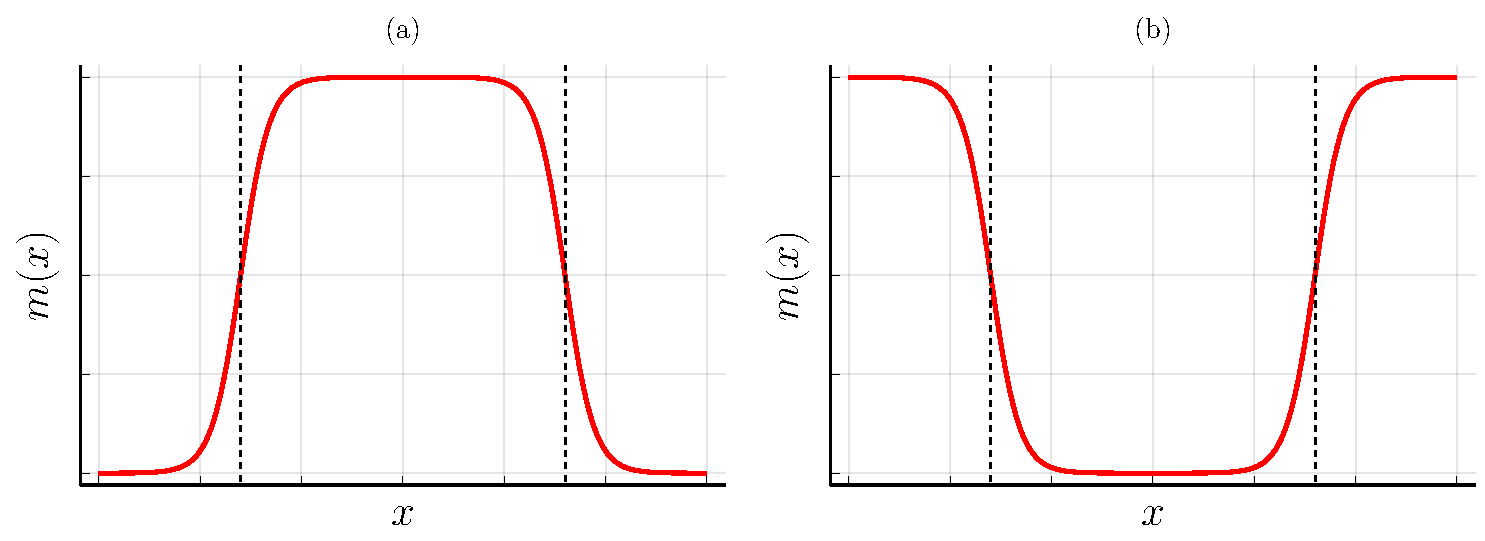
\includegraphics[width=\textwidth]{codes/twokink.pdf}
    \caption{(a) Kink-antikink pair (b)Antikink-kink pair}
\end{figure}
\noindent
Such kink and anti-kink pairs are deformable and annihilate each other as seen previously. 